% ----------------------------------------------------------
\chapter{Solução Proposta e Metodologia Utilizada}\label{cap:solucao_proposta}
% ----------------------------------------------------------

Este capítulo tratará da solução proposta e metodologia utilizada, bem como soluções alternativas que foram consideradas e descartadas ao longo do processo de proposta de uma solução para o problema considerado.


% \textbf{Instruções da Coordenação do PFC:}

% Neste capítulo, deve-se apresentar:
% \begin{itemize}
% 	\item A solução proposta para o problema descrito no capítulo anterior;
% 	\item Explicar a metodologia utilizada na solução proposta;
% 	\item Deixar bem claro e justificar tecnicamente para o leitor como que a solução proposta resolve o problema abordado e atende aos requisitos técnicos, explicando tecnicamente as decisões que foram tomadas para se chegar a tal solução.
% \end{itemize}

% Sugere-se colocar uma diagrama/fluxograma/casos de uso/etc ilustrando a solução proposta, e depois explicar em detalhes cada parte/bloco do diagrama/fluxograma ao longo do texto. 

% Ressaltamos que, em princípio, há uma infinidade de soluções possíveis para o problema abordado no PFC. Desse modo, é preciso explicar detalhadamente e justificar tecnicamente a solução proposta no PFC.

\section{Solução Proposta}

\subsection{Visão Geral}
Para atender aos desafios identificados no \autoref{cap:descricao_problema_e_requisitos}, propõe-se o desenvolvimento de um sistema web baseado em \textit{cloud computing}, com uma abordagem de \textit{Software as a Service} (SaaS), voltado para o gerenciamento de reservas de quadras esportivas e integração com dispositivos IoT. Uma visão geral da arquitetura do sistema está demonstrada na \autoref{fig:arquitetura_geral}. Esse sistema será composto por um backend responsável por toda a lógica de negócios e armazenamento dos dados, e um frontend voltado para a interação com os clientes e a administração das quadras, o qual será desenvolvido em um projeto futuro, além de um banco de dados para armazenar informações da aplicação.

\begin{figure}[htp]
	\caption{\label{fig:arquitetura_geral}Arquitetura geral da aplicação.}
	\begin{center}
	  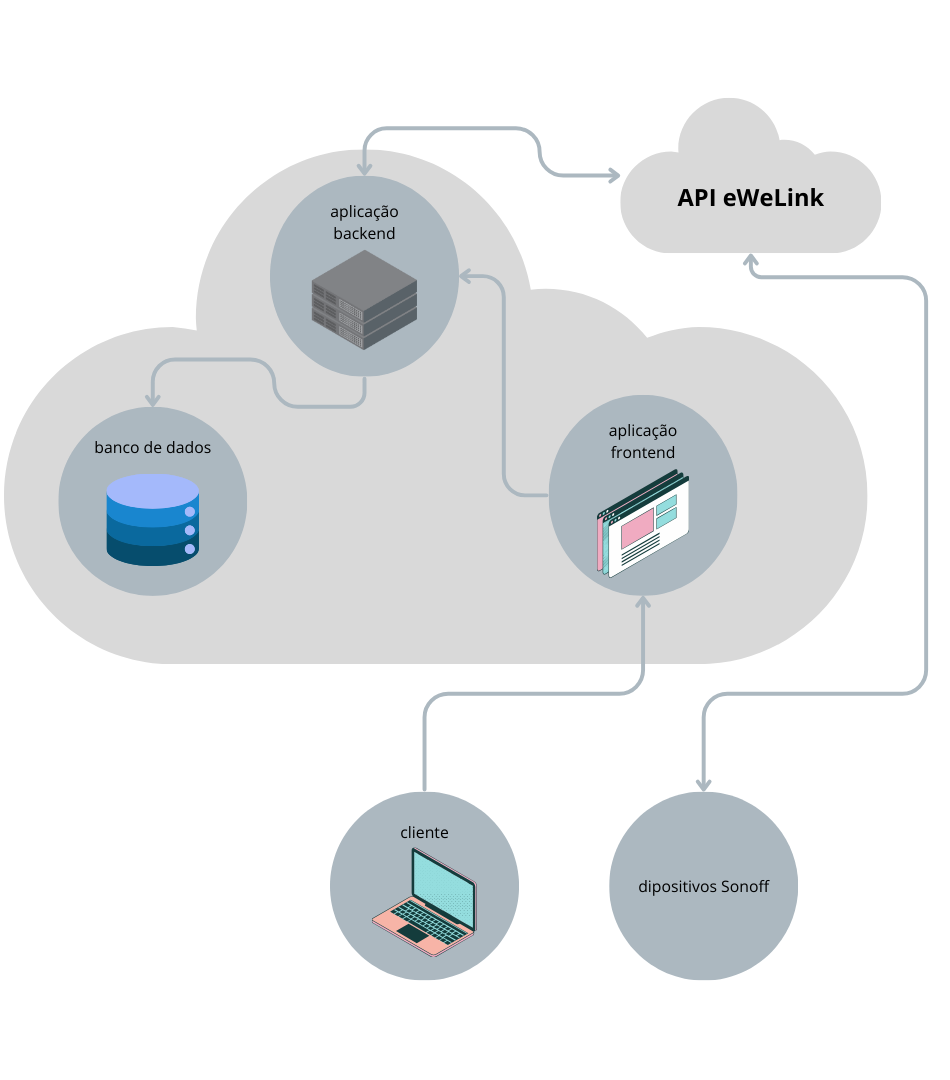
\includegraphics[scale=0.5]{images/cap4/arquitetura_geral.png}
	\end{center}
	\fonte{Autor.}
\end{figure}

O sistema adotará uma abordagem \textit{multi-tenant}, permitindo que múltiplas empresas utilizem a mesma plataforma de maneira independente. O administrador de cada empresa poderá configurar seu próprio ambiente, definindo nome, horários de funcionamento e quantidade de quadras disponíveis. Cada quadra terá horários de funcionamento ajustáveis de acordo com os dias da semana, garantindo flexibilidade na gestão.

Também foi considerada uma abordagem \textit{single-tenant} e replicável para cada cliente. O problema dessa abordagem é que a manutenção de cada instância do sistema seria mais custosa e complexa, pois cada cliente teria seu próprio banco de dados e instância do sistema. Além disso a necessidade de configuração manual para cada novo cliente seria trabalhosa e custosa para o time da Fischertec. A abordagem \textit{multi-tenant} é mais escalável e econômica, pois todos os clientes compartilham a mesma instância do sistema e banco de dados, com isolamento de dados e configurações.

Os clientes esportistas poderão acessar a plataforma para visualizar a disponibilidade das quadras de uma empresa em tempo real, selecionar um horário específico e realizar a reserva de forma simples e intuitiva. A confirmação das reservas será imediata por padrão, proporcionando uma experiência eficiente e conveniente tanto para os usuários quanto para os administradores. Será possível, também, configurar a necessidade de aprovação para as reservas, caso a empresa deseje revisar manualmente cada solicitação.

A fim de garantir a integração com dispositivos IoT de maneira simples e sem necessidade de conhecimento técnico por parte dos administradores das empresas, optou-se por utilizar uma solução de hardware consolidada no mercado, a Sonoff, que oferece dispositivos de automação residencial com suporte a integração via API. Dessa maneira, evita-se a necessidade de um hardware e uma aplicação extra que se conectaria ao servidor fazendo uma espécie de ponte para gerenciar os dispositivos IoT diretamente através da rede local. Além disso seria necessário uma configuração extra para liberar o controle local nos dispositivos Sonoff (o modo DIY \textit{Do It Yourself}) e atribuição de ips fixos na rede local (pois em caso de mudança de ip, seria necessário reconfigurar a aplicação de ponte para que ela pudesse encontrar os dispositivos na rede).

Portanto, a automação do controle dos dispositivos IoT será feita por meio da integração com a plataforma eWeLink, amplamente utilizada no mercado e compatível com dispositivos da marca Sonoff. O administrador poderá conectar sua conta eWeLink ao sistema, permitindo a identificação automática dos dispositivos configurados. Esses dispositivos poderão ser atribuídos às quadras e configurados para executar comandos específicos no início e/ou fim de uma reserva, como ligar ou desligar iluminação e climatização de forma automatizada. Essa solução permitirá que os administradores da empresa configurem facilmente os dispositivos IoT para funcionarem em conjunto com a plataforma, sem a necessidade de contatar profissionais de tecnologia ou executar instruções complexas, reduzindo a abertura de chamados de suporte da aplicação.

Com essa abordagem, o sistema proporcionará um gerenciamento eficiente e automatizado das quadras esportivas, reduzindo desperdícios, otimizando recursos e melhorando a experiência dos clientes. Além disso, a solução contribuirá para a redução de custos operacionais e impacto ambiental, tornando-se uma ferramenta indispensável para empresas que buscam modernização e eficiência em sua gestão.

O desenvolvimento do sistema completo será dividido em duas etapas: backend e frontend. Neste projeto de fim de curso, será abordada a implementação do backend, que consiste na construção de uma aplicação de servidor responsável por toda a lógica de negócios e integração com a plataforma eWeLink. A aplicação será desenvolvida em Node.js, utilizando o framework Nest.js na linguagem Typescript, afim de satisfazer os requisitos técnicos apresentados. Terá suporte a cadastro, autenticação e autorização de usuários, persistência de dados em um banco de dados PostgreSQL e integração com a API da eWeLink.

